\documentclass[10pt]{article}
\usepackage{fullpage,enumitem,amsmath,amssymb,graphicx,listings,tikz,bbm,xcolor,algorithm2e,hyperref}
\setlength{\parindent}{0pt}

\begin{document}

\begin{center}
{\Large \textbf{Theory Problems}}

\begin{tabular}{rl}
\\
Course: & Coursera Algorithms Specialization \\
Name: & Bryan Yaggi
\end{tabular}
\end{center}

\section*{\normalsize Problem 1}

In the 2SAT problem, you are given a set of clauses, where each clause is the disjunction of two literals (a literal is a Boolean variable or the negation of a Boolean variable). You are looking for a way to assign a value "true" or "false" to each of the variables so that all clauses are satisfied --- that is, there is at least one true literal in each clause. For this problem, design an algorithm that determines whether or not a given 2SAT instance has a satisfying assignment. (Your algorithm does not need to exhibit a satisfying assignment, just decide whether or not one exists.) Your algorithm should run in $O(m+n)$ time, where $m$ and $n$ are the number of clauses and variables, respectively. [Hint: strongly connected components.]
\bigskip

Each clause, a disjunction of 2 literals, can be represented as 2 implications. These implications can be used to create an implication graph. If the implication graph has any cycles containing a variable and its negation, a contradiction exists and therefore no satisfying assignment exists. Kosaraju's algorithm can be used to find the strongly connected components of a graph. It uses two depth-first searches, so it has $O(m + n)$ complexity. If a variable and its negation are present in the same strongly connected component, no satisfying assignment exists. 
\smallskip

Example: Given $(x_1 \vee x_2) \wedge (\neg x_2 \vee x_3) \wedge (x_3 \vee x_4) \wedge (\neg x_3 \vee x_5) \wedge (\neg x_4 \vee \neg x_5) \wedge (\neg x_3 \vee x_4) \wedge (\neg x_1 \vee \neg x_2)$

\begin{align*}
  (x_1 \vee x_2) &\leftrightarrow (\neg x_1 \rightarrow x_2) \wedge (\neg x_2 \rightarrow x_1) \\
  (\neg x_2 \vee x_3) &\leftrightarrow (x_2 \rightarrow x_3) \wedge (\neg x_3 \rightarrow \neg x_2) \\
  (x_3 \vee x_4) &\leftrightarrow (\neg x_3 \rightarrow x_4) \wedge (\neg x_4 \rightarrow x_3) \\
  (\neg x_3 \vee x_5) &\leftrightarrow (x_3 \rightarrow x_5) \wedge (\neg x_5 \rightarrow \neg x_3) \\
  (\neg x_4 \vee \neg x_5) &\leftrightarrow (x_4 \rightarrow \neg x_5) \wedge (x_5 \rightarrow \neg x_4) \\
  (\neg x_3 \vee x_4) &\leftrightarrow (x_3 \rightarrow x_4) \wedge (\neg x_4 \rightarrow \neg x_3) \\
  (\neg x_1 \vee \neg x_2) &\leftrightarrow (x_1 \rightarrow \neg x_2) \wedge (x_2 \rightarrow \neg x_1)
\end{align*}

\begin{center}
  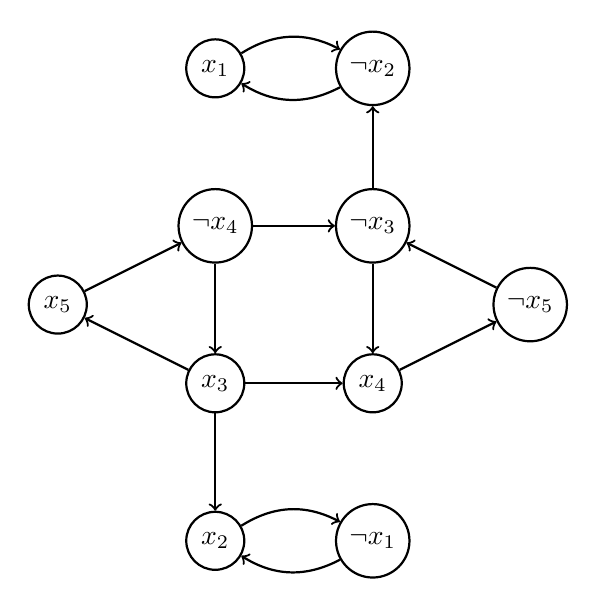
\begin{tikzpicture}
    \begin{scope}[every node/.style={circle,thick,draw}]
      \node (X1)  at (-1, 3) {$x_1$};
      \node (X2n) at ( 1, 3) {$\neg x_2$};
      \node (X4n) at (-1, 1) {$\neg x_4$};
      \node (X3n) at ( 1, 1) {$\neg x_3$};
      \node (X5)  at (-3, 0) {$x_5$};
      \node (X5n) at ( 3, 0) {$\neg x_5$};
      \node (X3)  at (-1,-1) {$x_3$};
      \node (X4)  at ( 1,-1) {$x_4$};
      \node (X2)  at (-1,-3) {$x_2$};
      \node (X1n) at ( 1,-3) {$\neg x_1$};
    \end{scope}
    \begin{scope}[every edge/.style={draw=black,thick}]
      \path [->, bend left] (X1)  edge node {} (X2n);
      \path [->, bend left] (X2n) edge node {} (X1);
      \path [->]            (X3n) edge node {} (X2n);
      \path [->]            (X4n) edge node {} (X3n);
      \path [->]            (X4n) edge node {} (X3);
      \path [->]            (X3n) edge node {} (X4);
      \path [->]            (X3)  edge node {} (X4);
      \path [->]            (X3)  edge node {} (X2);
      \path [->, bend left] (X1n) edge node {} (X2);
      \path [->, bend left] (X2)  edge node {} (X1n);
      \path [->]            (X5)  edge node {} (X4n);
      \path [->]            (X3)  edge node {} (X5);
      \path [->]            (X4)  edge node {} (X5n);
      \path [->]            (X5n) edge node {} (X3n);
    \end{scope}
  \end{tikzpicture}
\end{center}

A satisfying assignment exists.

\section*{\normalsize Problem 2}

In lecture we define the length of a path to be the sum of the lengths of its edges. Define the bottleneck of a path to be the maximum length of one of its edges. A mininum-bottleneck path between two vertices $s$ and $t$ is a path with bottleneck no larger than that of any other $s-t$ path. Show how to modify Dijkstra's algorithm to compute a minimum-bottleneck path between two given vertices. The running time should be $O(m \log ⁡n)$, as in lecture.
\bigskip

Dijkstra's algorithm can be modified so that the value stored in the priority queue (minimum heap) is the bottleneck instead of the total path length. Dijkstra's running time is $O(m \log n)$.

\section*{\normalsize Problem 3}

We can do better. Suppose now that the graph is undirected. Give a linear-time $O(m)$ algorithm to compute a minimum-bottleneck path between two given vertices.
\bigskip

Camerini's algorithm finds the minimum bottleneck spanning tree in $O(m)$. The minimum bottleneck path between any two vertices will follow the minimum bottleneck spanning tree between those two vertices. See Wikipedia article on Minimum Bottleneck Spanning Trees.

\section*{\normalsize Problem 4}

What if the graph is directed? Can you compute a minimum-bottleneck path between two given vertices faster than $O(m \log n)$ ?
\bigskip

Camerini's algorithm for directed graphs finds the minimum bottleneck spanning arborescence, a directed graph from source vertex to each of the other connected vertices, in $O(m \log m)$. Gabow and Tarjan's algorithm for minimum bottleneck spanning arborescence uses the modified version of Dijkstra's algorithm mentioned in Problem 2 and implements the priority queue using a Fibonacci heap. It runs in $O(m + n log n)$. See Wikipedia article on Minimum Bottleneck Spanning Trees.

\section*{\normalsize Problem 5}

Recall that a set $H$ of hash functions (mapping the elements of a universe $U$ to the buckets ${0,1,2,\dots,n-1}$) is universal if for every distinct $x,y \in U$, the probability $Prob[h(x) = h(y)]$ that $x$ and $y$ collide, assuming that the hash function $h$ is chosen uniformly at random from $H$, is at most $\frac{1}{n}$. In this problem you will prove that a collision probability of $\frac{1}{n}$ is essentially the best possible. Precisely, suppose that $H$ is a family of hash functions mapping $U$ to ${0,1,2,\dots,n-1}$, as above. Show that there must be a pair $x,y \in U$ of distinct elements such that, if $h$ is chosen uniformly at random from $H$, then $Prob[h(x) = h(y)] \geq \frac{1}{n} - \frac{1}{|U|}$
\bigskip

Answer...

\end{document}
